\section{Giải pháp thực hiện}    
    Đồ án này tập trung vào việc phát triển một hệ thống hỗ trợ quyết định trên nền tảng website, sử dụng mô hình Ikigai để hỗ trợ sinh viên lựa chọn ngành học và nghề nghiệp. Mục tiêu chính của hệ thống \acrshort{dss} này là giúp sinh viên khám phá đam mê, thế mạnh và cách chuyển đổi những yếu tố này sao cho phù hợp với nhu cầu của xã hội, từ đó thúc đẩy việc ra các quyết định sáng suốt về con đường học vấn và nghề nghiệp .

    Phương pháp được áp dụng để mô hình hóa là sơ đồ Venn Ikigai bao gồm 4 câu hỏi: ``Bạn yêu thích điều gì", ``Bạn giỏi điều gì", ``Bạn được trả lương để làm gì", và ``Thế giới cần gì". 
    \begin{figure}[H]
        \centering
        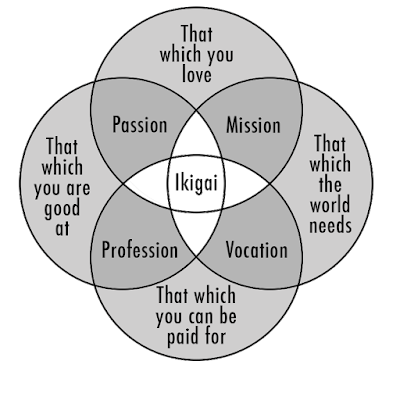
\includegraphics[width=0.5\linewidth]{images/ikigai.png}
        \vspace{0.6cm}
        \caption{Sơ đồ venn Ikigai}
    \end{figure}

    Mỗi câu hỏi được giải quyết bằng các phương pháp giải khác nhau được thiết kế riêng sau đó dựa trên Phân tích Quyết định Đa tiêu chí (Multiple-criteria decision-making - \acrshort{mcdm} hoặc Multiple-criteria decision analysis - \acrshort{mcda}) để tính toán, và tổng hợp kết quả. Trắc nghiệm tính cách Myers-Briggs Type Indicator (\acrshort{mbti}) được sử dụng để hiểu sở thích của người dùng cho câu hỏi ``Bạn yêu thích điều gì," trong khi phân vùng nhóm ngành nghề (Career Clustering) giúp phân loại người dùng vào các nhóm ngành dựa trên thế mạnh, từ đó trả lời cho câu hỏi ``Bạn giỏi gì". Dữ liệu từ nhiều nguồn uy tín khác nhau như Tổng cục thống kê, LinkedIn, Career Viet Data, các trang web, công văn của chính phủ được sử dụng để phân tích mức lương và nhu cầu cho câu hỏi ``Bạn được trả lương để làm gì?" và ``Thế giới cần gì?".
    
    Tiếp theo đó, sử dụng các phương pháp trong phân tích quyết định đa tiêu chí để tìm được giải pháp phù hợp nhất. Trong đồ án này sử dụng 2 phương pháp để tìm ra tiêu chí phù hợp.
    
    Phương pháp đầu tiên được áp dụng là Vikor(VišeKriterijumska Optimizacija i Kompromisno Rešenje) được phát triển bởi Srdjan M. Opricovic vào năm 1998. Phương pháp này được sử dụng để lựa chọn giải pháp tối ưu từ nhiều lựa chọn có cùng tiêu chí đánh giá. VIKOR xác định giải pháp thỏa hiệp, là giải pháp gần với lý tưởng nhất và có sự đồng thuận cao nhất giữa các tiêu chí. Ưu điểm của VIKOR là VIKOR không chỉ tìm ra giải pháp tốt nhất theo từng tiêu chí mà còn xác định giải pháp cân bằng giữa các tiêu chí, phù hợp với thực tế. Tuy vậy VIKOR cũng tồn tại những nhược điểm về mức ảnh hưởng của các trọng số, do đó cần cân nhắc kỹ lưỡng khi lựa chọn. VIKOR có thể được áp dụng cho nhiều loại vấn đề khác nhau với nhiều tiêu chí đánh giá như là đầu tư, kinh doanh, lựa chọn nhân sự, bệnh án,...

    Ngoài ra, hệ hỗ trợ còn sử dụng một phương pháp đơn giản là Weighted sum (tổng trọng số). Phương pháp này hoạt động bằng cách gán trọng số cho từng tiêu chí và tính toán tổng điểm cho mỗi lựa chọn dựa trên giá trị của nó đối với từng tiêu chí. Lựa chọn có tổng điểm cao nhất được coi là giải pháp tối ưu. Tuy đơn giản nhưng phương pháp này lại ẩn chứa nhiều rủi ro khi kết quả của Weighted Sum phụ thuộc rất nhiều vào trọng số được gán cho các tiêu chí. Do đó, việc lựa chọn trọng số phù hợp là rất quan trọng và có thể ảnh hưởng đến kết quả cuối cùng, cũng như việc Weighted sum giả định rằng mối quan hệ giữa các tiêu chí là tuyến tính. Tuy nhiên, trong thực tế, mối quan hệ giữa các tiêu chí có thể không phải lúc nào cũng tuyến tính. Tuy vậy, đây là phương pháp cơ bản, nền tảng cho \acrshort{mcdm} nên nhóm vẫn quyết định thực hiện phương pháp này.
    
    Sau khi tính toán và xếp hạng, hệ thống dựa vào cơ sở dữ liệu để đưa ra gợi ý cho người dùng về những định hướng trong nghề nghiệp, ngành học. Đây cũng là quá trình mô phòng lại việc tìm kiếm ikigai - lý do để sống ở ngoài thực tế. Chúng ta cũng sẽ tìm hiểu, đánh giá mức độ phù hợp, trải nghiệm thử và từ đó đưa ra quan điểm, lựa chọn mà bản thân cảm thấy đúng đắn và hợp lý nhất.
    
    Thông qua quyết định được gợi ý từ hệ thống DSS, người dùng có thể có được thông tin đa dạng, có những hiểu biết sâu sắc hơn về đam mê, thế mạnh và con đường nghề nghiệp tiềm năng của mình, từ đó dẫn đến sự tự tin hơn trong quá trình ra quyết định cho mỗi cá nhân. Các phương pháp Vikor, Weighted sum được áp dụng trong bài toán \acrshort{mcdm} nhằm cân bằng giữa các tiêu chí để đưa ra giải pháp cân bằng giữa các yếu tố, đó cũng là điều mà mô hình Ikigai hướng đến.